\section{Introduction}\label{sec:intro}
Transformer~\cite{vaswani2017attention} has been dominant in deep learning research for recent years. 
It works as a backbone module in many fundamental models, achieving outstanding performance in various application scenarios. 
Currently, the most successful language models like BERT~\cite{devlin2019bert} and GPT~\cite{brown2020language} are built based on the Transformer or its variants~\cite{child2019generating,dai2019transformer}, which outperforms classic recurrent neural network (RNN) architectures on both effectiveness and efficiency. 
In the field of computer vision, the Vision Transformers (ViTs)~\cite{dosovitskiy2021an,liu2021swin,arnab2021vivit} have achieved better performance in many image recognition and understanding tasks compared to convolutional neural networks (CNNs).
Recently, the Transformer-based models have been designed for the structured data in different applications, including the Informer~\cite{zhang2021informer} for time series broadcasting, the Graphormer~\cite{ying2021transformers} for molecular representation, the Set-Transformer~\cite{lee2019set} and Point-Transformer~\cite{zhao2021point} for point cloud modeling, and so on.
More and more cases show the tendency that the Transformer is becoming an indispensable choice when developing deep learning models.

\begin{table}[t]
    \caption{A comparison for representative Transformers and our Sliceformer on their attention mechanisms. 
    We show one attention head for each transformer, in which the input $\bm{X}\in\mathbb{R}^{N\times d}$, the value $\bm{V}=\bm{X}\bm{W}_V\in\mathbb{R}^{N\times D}$, the query $\bm{Q}=\bm{X}\bm{W}_Q\in\mathbb{R}^{N\times D}$, and the key $\bm{K}=\bm{X}\bm{W}_K\in\mathbb{R}^{N\times D}$.}
    \label{tab:cmp}
    \centering
    \small{
    \begin{threeparttable}
    {\def\arraystretch{1.3}\tabcolsep=4pt
    \begin{tabular}{l|lll}
    \toprule
    Model & 
    $\text{Attention}(\bm{V};\bm{Q},\bm{K})$ & 
    Complexity & 
    Attention Structure \\
    \midrule
    Transformer~\cite{vaswani2017attention}  & 
    $\text{Softmax}\left(\frac{\bm{Q}\bm{K}^{\top}}{\sqrt{D}}\right)\bm{V}$ & 
    $\mathcal{O}(DN^2)$ & 
    Dense + Row-stochastic\\
    SparseTrans~\cite{child2019generating} & 
    $\text{Local2D-Softmax}\left(\frac{\bm{Q}\bm{K}^{\top}}{\sqrt{D}}\right)\bm{V}$ & 
    $\mathcal{O}(DN^{1.5})$ &
    Sparse + Row-stochastic\\
    Longformer~\cite{beltagy2020longformer}   & 
    $\text{Local1D-Softmax}\left(\frac{\bm{Q}\bm{K}^{\top}}{\sqrt{D}}\right)\bm{V}$ &  
    $\mathcal{O}(DNL)$ &
    Sparse + Row-stochastic\\
    Reformer~\cite{kitaev2020reformer}     & 
    $\text{LSH-Softmax}\left(\frac{\bm{Q}\bm{K}^{\top}}{\sqrt{D}}\right)\bm{V}$ &  
    $\mathcal{O}(DN\log N)$ &
    Sparse + Row-stochastic\\
    CosFormer~\cite{zhen2022cosformer}    & 
    $(\bm{Q}_{\cos}\bm{K}_{\cos}^{\top}+\bm{Q}_{\sin}\bm{K}_{\sin}^{\top})\bm{V}$ & 
    $\mathcal{O}(\min\{DE_{QK},NE_{Q}\})$&
    Sparse\\
    Performer~\cite{choromanski2021rethinking}  & 
    $\phi_r(\bm{Q})\phi_r(\bm{K})^{\top}\bm{V}$ & 
    $\mathcal{O}(DNr)$ &
    Low-rank\\
    Linformer~\cite{wang2020linformer}    & 
    $\text{Softmax}\left(\frac{\bm{Q}\psi_r(\bm{K})^{\top}}{\sqrt{D}}\right)\psi_r(\bm{V})$ & 
    $\mathcal{O}(DNr)$ &
    Low-rank + Row-stochastic\\
    Sinkformer~\cite{sander2022sinkformers}   & 
    $\text{Sinkhorn}_{K}\left(\frac{\bm{Q}\bm{K}^{\top}}{\sqrt{D}}\right)\bm{V}$ & 
    $\mathcal{O}(KDN^2)$ &
    Dense + Doubly stochastic\\
    \midrule
    \multirow{2}{*}{\textbf{Sliceformer}}  & 
    \multirow{2}{*}{$\text{Sort}_{\text{col}}(\bm{V})$} & 
    \multirow{2}{*}{$\mathcal{O}(DN\log N)$} &
    Full-rank + Sparse\\
    &
    &
    &
    + Doubly stochastic\\
    \bottomrule
    \end{tabular}
    }
    \begin{tablenotes}
    \item[1] \footnotesize{``Local1D'' considers $L$ local data in a sequence. ``Local2D'' considers the row-wise and column-wise local data for a sequence zigzagging in the 2D space. ``LSH'' denotes Locality-sensitive Hashing.}
    \item[2] \footnotesize{$\phi_r: \mathbb{R}^{D}\mapsto\mathbb{R}^r$, and $\phi_r(\bm{Q}),\phi_r(\bm{K})\in\mathbb{R}^{N\times r}$; $\psi_r: \mathbb{R}^{N}\mapsto\mathbb{R}^r$, and $\psi_r(\bm{K}),\psi_r(\bm{V})\in\mathbb{R}^{r\times D}$.}
    \item[3] $\bm{K}_{\cos}=\text{diag}(\{\cos\frac{\pi i}{2M}\}_{i=1}^{N})\text{ReLU}(\bm{K})$, $\bm{K}_{\sin}=\text{diag}(\{\sin\frac{\pi i}{2M}\}_{i=1}^{N})\text{ReLU}(\bm{K})$. So are $\bm{Q}_{\cos}$ and $\bm{Q}_{\sin}$. 
    $E_{QK}$ is the number of nonzero elements in $\bm{Q}_{\cos}\bm{K}_{\cos}^{\top}$. $E_Q$ is the number of nonzero elements in $\bm{Q}_{\cos}$.
    \item[4] ``$\text{Sinkhorn}_{K}$'' means applying $K$-step Sinkhorn iterations.
    \item[5] Note that, our Sliceformer does not need the ``multi-head'' architecture because of the simplicity of sorting.
    \end{tablenotes}
    \end{threeparttable}
}
\end{table}


Although without strict theoretical support, the effectiveness of the Transformer is often attributed to the multi-head attention (MHA) mechanism~\cite{vaswani2017attention} behind it.
This empirical but dominant opinion impacts the design and modification of the Transformer significantly, which, in our opinion, might have restricted the development of new model architectures to some degree.
As shown in Table~\ref{tab:cmp}, 
\begin{wrapfigure}{r}{0.5\textwidth}
  \centering
    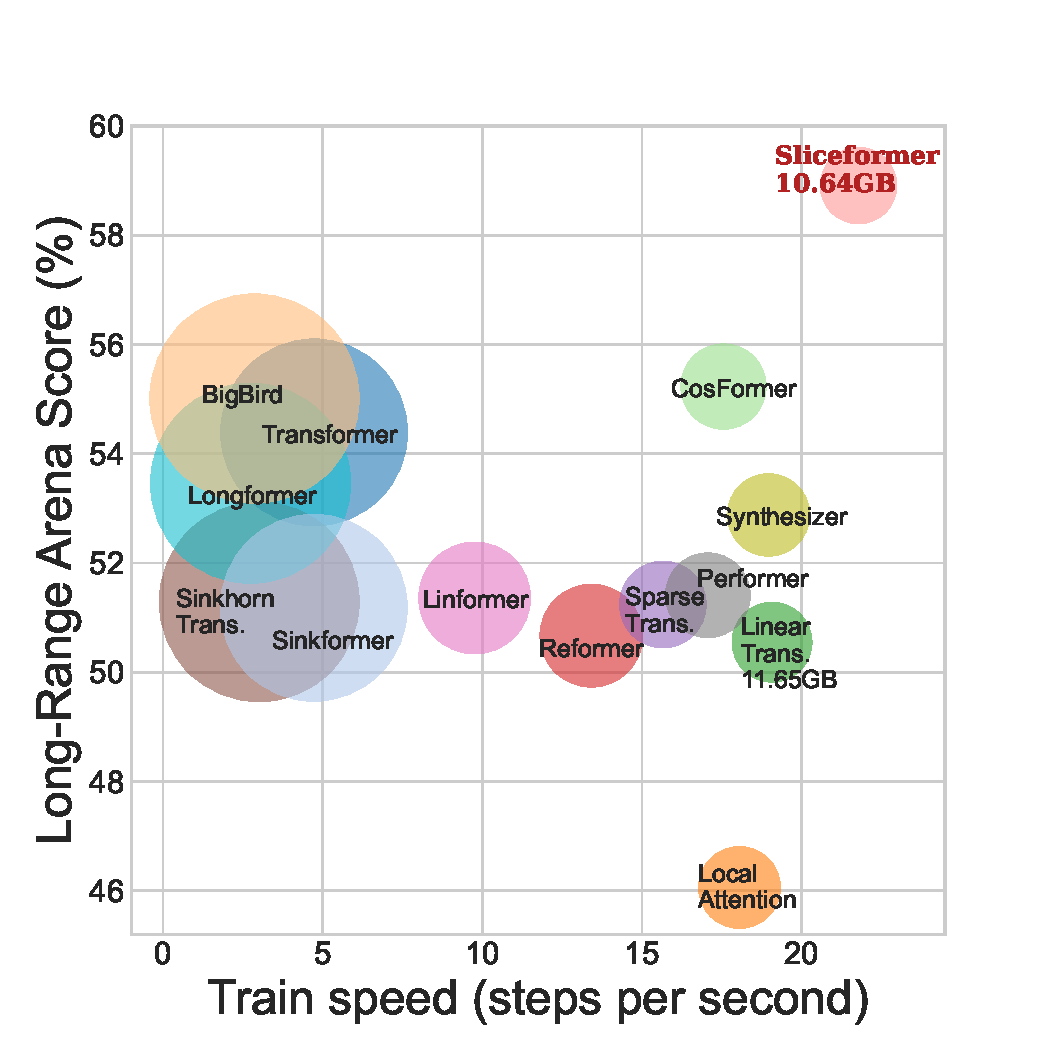
\includegraphics[width=0.46\textwidth]{figures/lra-3.pdf}
    \caption{The comparison for various Transformers and our Sliceformer on the LRA benchmark. 
    The length of the sequence is 3K.
    The x-axis corresponds to the number of training steps per second. 
    The y-axis corresponds to the average score (\%) on the LRA benchmark.
    The peak memory usage of each model is represented as the area of the corresponding circle. 
    For a better comparison, the values (GB) of the top-2 models are shown.}
    \label{fig:cmp}
\end{wrapfigure}
many variants of Transformer have been proposed to $i)$ improve the efficiency of MHA (e.g., designing sparse or low-rank attention maps~\cite{child2019generating,kitaev2020reformer,wang2020linformer}), $ii)$ enhance the interpretability of MHA (e.g., revisiting attention maps through the lens of kernel theory~\cite{tsai2019transformer,zhen2022cosformer} and optimal transport~\cite{tay2020sparse,sander2022sinkformers}), or $iii)$ impose more side information on attention maps~\cite{dong2021attention,ying2021transformers,ma2022mega}. 
However, they still rely on the classic ``query-key-value'' architecture of MHA. 
Little attention is paid to studying the necessity of the MHA itself or, more ambitiously, replacing the MHA with a new surrogate. 
Some work replaces the MHA with some other architectures, e.g., RNN~\cite{katharopoulos2020transformers}, MLP~\cite{tolstikhin2021mlp}, and Structured State Space Sequential Model~\cite{gu2021efficiently}. 
Still, they mainly focus on reusing existing neural networks in specific tasks rather than designing a new and general module.



In this study, we challenge the architecture of MHA, replacing it with an extremely simple ``slicing-sorting'' operation and developing a surrogate of the Transformer called Sliceformer. 
In particular, our work is motivated by the MHA's drawbacks and the attention map's possibly-desired structure. 
Firstly, we attribute the MHA's numerical issues to the softmax operation and point out the potential loss of model capacity caused by the multi-head structure. 
Secondly, the development tendency of the MHA and its variants implies that we shall pursue as many sparse and doubly stochastic attention maps as possible for projected samples. 
Based on the analysis above, we propose the ``slicing-sorting'' operation, which projects samples linearly to a latent space and sorts them along different feature dimensions. 
Replacing the MHA mechanism of the Transformer with the slicing-sorting operation leads to the proposed Sliceformer.



As shown in Table~\ref{tab:cmp}, our slicing-sorting operation only preserves the linear map from the input $\bm{X}$ to the value matrix $\bm{V}$. 
In addition, we do not need the ``multi-head'' structure because concatenating different linear maps is equivalent to increasing the columns of $\bm{W}_V$ directly. 
Therefore, our Sliceformer has fewer parameters and lower computational complexity than the Transformer and its variants. 
We analyze the connections and differences between the proposed slicing-sorting operation and the MHA mechanism and discuss its rationality in depth. 
Specifically, we find that although abandoning the MHA architecture, the slicing-sorting operation achieves sparse and doubly stochastic attention maps by a set of permutation matrices. 
We test our Sliceformer in the well-known Long-Range Arena (LRA) benchmark. 
As shown in Figure~\ref{fig:cmp}, our Sliceformer achieves superior performance with less memory cost and runtime compared to the Transformer and its variants. 
Moreover, through other discriminative learning tasks like image classification and molecular analysis, we further demonstrate the universal applicability of our Sliceformer and highlight its advantage in numerical stability.